\documentclass[11pt]{article}
\usepackage[margin=2.2cm]{geometry}
\usepackage{amsmath,amssymb,graphicx,booktabs,hyperref,xcolor}
\usepackage[font=small]{caption}
\usepackage{url}
\newcommand{\Mee}{M_{ee}}
\newcommand{\Jpsi}{J/\psi}
\title{The $M(e^+e^-)$ lineshape of $\Jpsi\to e^+e^-(\gamma)$:\\
a corrected fit function and how to use it}
\author{J/$\psi$ electroproduction RC session, for V.~Kubarovsky}
\date{9 October 2026}
\begin{document}
\maketitle

\begin{abstract}
The function \texttt{dNdMee.cpp} describes the $e^+e^-$ invariant-mass spectrum of
$\Jpsi\to e^+e^-(\gamma)$ with three parameters: the peak position $M$, a Gaussian
resolution $\sigma$, and the fraction \texttt{br} of decays with a photon above
$\varepsilon=1$~MeV.  Fitted to the generator's own $\Jpsi$ decays it finds $M$
exactly, but its tail is off by up to 20\,\% and, folded with a 30~MeV resolution,
it returns a $\Jpsi$ yield 2.5\,\% too low and $M$ 0.7~MeV too high with a perfectly
acceptable $\chi^2$ --- an error a fit to data cannot reveal.  Three causes are
identified: the photon energy is taken as $M-\Mee$ instead of
$k=(M^2-\Mee^2)/2M$, the spectrum is first order instead of exponentiated, and its
normalisation constant is 3\,\% off.  A corrected function \texttt{dNdMee\_v2.cpp},
with the same interface, agrees with the generator to five digits, returns $M$,
$\sigma$ and the yield without bias, and does not depend on $\varepsilon$.  The
recommendation for data is to keep the radiative part fixed by QED and fit only the
yield, the mass scale and the resolution; the detector response beyond a Gaussian is
the next step, with GEMC.
\end{abstract}

\section{The spectrum}

In the $\Jpsi$ rest frame a photon of energy $k$ leaves the pair with
\begin{equation}
  \Mee^2 = M^2 - 2Mk ,\qquad k = \frac{M^2-\Mee^2}{2M},\qquad
  \frac{dk}{d\Mee} = \frac{\Mee}{M}.
  \label{eq:kin}
\end{equation}
To first order in $\alpha$ the photon spectrum is (Ehlotzky and Mitter, $E=M/2$, $x=k/E$)
\begin{equation}
  \frac{1}{\Gamma_0}\frac{d\Gamma}{dk} =
  \frac{2\alpha}{\pi}\Big[2\ln\Big(\frac{2E}{m_e}\sqrt{1-x}\Big)-1\Big]
  \frac{1}{k}\Big(1-x+\frac{x^2}{2}\Big),
  \label{eq:em}
\end{equation}
and the correction with all photons below $K$ (soft and virtual included) has the
closed form $\delta(K)$ of \texttt{rc\_vector\_mesons.py:delta\_vm}, with
$d\delta/dK$ equal to Eq.~(\ref{eq:em}).  The leading logarithm,
$\delta(K)\simeq\beta\ln(K/E)$ with
\begin{equation}
  \beta=\frac{2\alpha}{\pi}\Big(\ln\frac{M^2}{m_e^2}-1\Big)=0.0763,
\end{equation}
is exponentiated, giving the cumulative distribution of the photon energy
\begin{equation}
  F(K) = \Big(\frac{K}{E}\Big)^{\beta}\,
  \frac{1+\delta(K)-\beta\ln(K/E)}{1+\delta(E)},\qquad F(E)=1 .
  \label{eq:F}
\end{equation}
$F$ is normalised to the radiation-inclusive width: the measured
$\mathcal B(\Jpsi\to e^+e^-)$ counts $e^+e^-(\gamma)$ (BESIII restores the tail below
its 2.7~GeV window with PHOTOS), so the lineshape is a probability density and carries
no factor $1+\delta$.  This is exactly what the event generator samples
(\path{exclurad_py/generator/decay_rad.py}); its angular part, the exact
tree-level matrix element, does not affect $\Mee$.  Two useful numbers:
$1-F(1~\text{MeV}) = 0.3945$ of the decays have a photon above 1~MeV, and
$P(\Mee<3.0~\text{GeV}) = 0.1466$.

\section{What is wrong with \texttt{dNdMee.cpp}}

The original function uses Eq.~(\ref{eq:em}) with $k$ replaced by $x=M-\Mee$, a
Gaussian peak of weight $1-\mathtt{br}$, and the tail scaled by
$\mathtt{br}\times\mathtt{Norm}$, $\mathtt{Norm}=2.0707$.  Three points:
\begin{enumerate}
\item \textbf{Wrong variable.}  $M-\Mee$ is not the photon energy; with
  Eq.~(\ref{eq:kin}), $k=(M-\Mee)(M+\Mee)/2M$, smaller by up to 20\,\% at
  $\Mee\simeq2$~GeV, and a density in $\Mee$ needs the Jacobian $\Mee/M$.
\item \textbf{First order.}  The $1/k$ spectrum has too many photons just above
  $\varepsilon$; the exponentiated $k^{\beta-1}$ shape matters because
  $\varepsilon=1$~MeV is deep in the soft region.
\item \textbf{Normalisation.}  $\int_{1\,\text{MeV}}^{E}$ of Eq.~(\ref{eq:em}) is
  0.4984, so the normalising constant should be 2.0066, not 2.0707: the tail is
  normalised to 1.032.
\end{enumerate}
Fig.~\ref{fig:spec} compares the two unfolded tails at the same \texttt{br}: the
original is 5--10\,\% low over most of the range and up to 35\,\% high next to the peak.

\begin{figure}[h]
\centering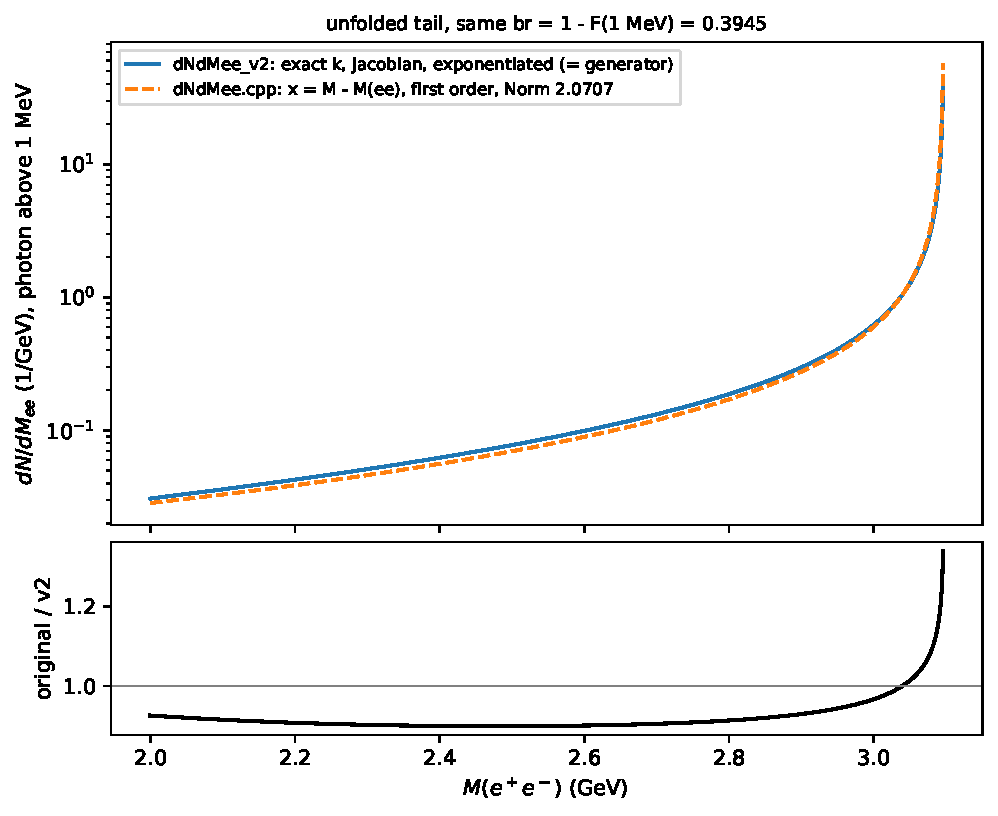
\includegraphics[width=0.66\textwidth]{figures/fig_spectrum_compare.pdf}
\caption{Unfolded $\Mee$ tail (photon above 1~MeV) of the corrected function
(= generator) and of the original formula, both with $\mathtt{br}=1-F(1~\text{MeV})$.}
\label{fig:spec}
\end{figure}

\section{The corrected function \texttt{dNdMee\_v2.cpp}}

Same call, \texttt{dNdMee(mee, M, sigma, br)}, plus a general
\texttt{dNdMee\_full(mee, M, sigma, br, eps, m)} (lepton mass $m$, so it also serves
$\mu^+\mu^-$).  It returns $dN/d\Mee$ in GeV$^{-1}$, normalised to one:
\begin{equation}
  \frac{dN}{d\Mee} = F(\varepsilon)\,G(\Mee-M;\sigma)
  + \frac{\mathtt{br}}{1-F(\varepsilon)}\int_{\varepsilon}^{k_{\max}}
  \frac{dF}{dk}\,G\big(\Mee-\sqrt{M^2-2Mk};\sigma\big)\,dk ,
\end{equation}
with $dF/dk$ from Eq.~(\ref{eq:F}) in closed form, the integral done in $\ln k$
(Simpson, 400 nodes, within $\pm8\sigma$).  \textbf{\texttt{br}~$<0$, the default,
means the QED value} $1-F(\varepsilon)$; a value in $[0,1]$ overrides it and is
meant for studies only.  $\sigma\le0$ returns the unfolded tail.  The code has no
dependence outside the C++ standard library and compiles also as a shared library
(used for every fit below, so the fits test the code a user will call).

Checks: $F(1~\text{MeV})=0.60551$, and $P(k>K)$ for $K=0.01$, 0.1, 0.3, 1~GeV
is 0.27855, 0.14368, 0.07724, 0.01590, identical to five digits to the generator;
$\int dN/d\Mee = 0.9965$ over 1.0--3.4~GeV at $\sigma=30$~MeV (the rest is below
1~GeV).

\section{Tests}

\subsection{MC truth, no resolution}
The generator's $\Mee$ (200k Born decays, no acceptance cut) fitted with
$\sigma=0.1$~MeV fixed and $N$, $M$, \texttt{br} free (Fig.~\ref{fig:truth},
0.2~MeV bins at the peak; $\chi^2$ excludes the 1.2~MeV next to the peak, which a
0.1~MeV Gaussian cannot describe for a delta):

\begin{center}
\begin{tabular}{lccc}\toprule
model & $M$ (GeV) & \texttt{br} & $\chi^2$/ndf\\\midrule
original \texttt{dNdMee.cpp} & 3.096900 & $0.3802\pm0.0011$ & 1302/215\\
exact $k$ + exponentiated (= v2) & 3.096900 & $0.3944\pm0.0011$ & 202/215\\
counted in the sample & 3.0969 & 0.3946 & \\\bottomrule
\end{tabular}
\end{center}

\begin{figure}[h]
\centering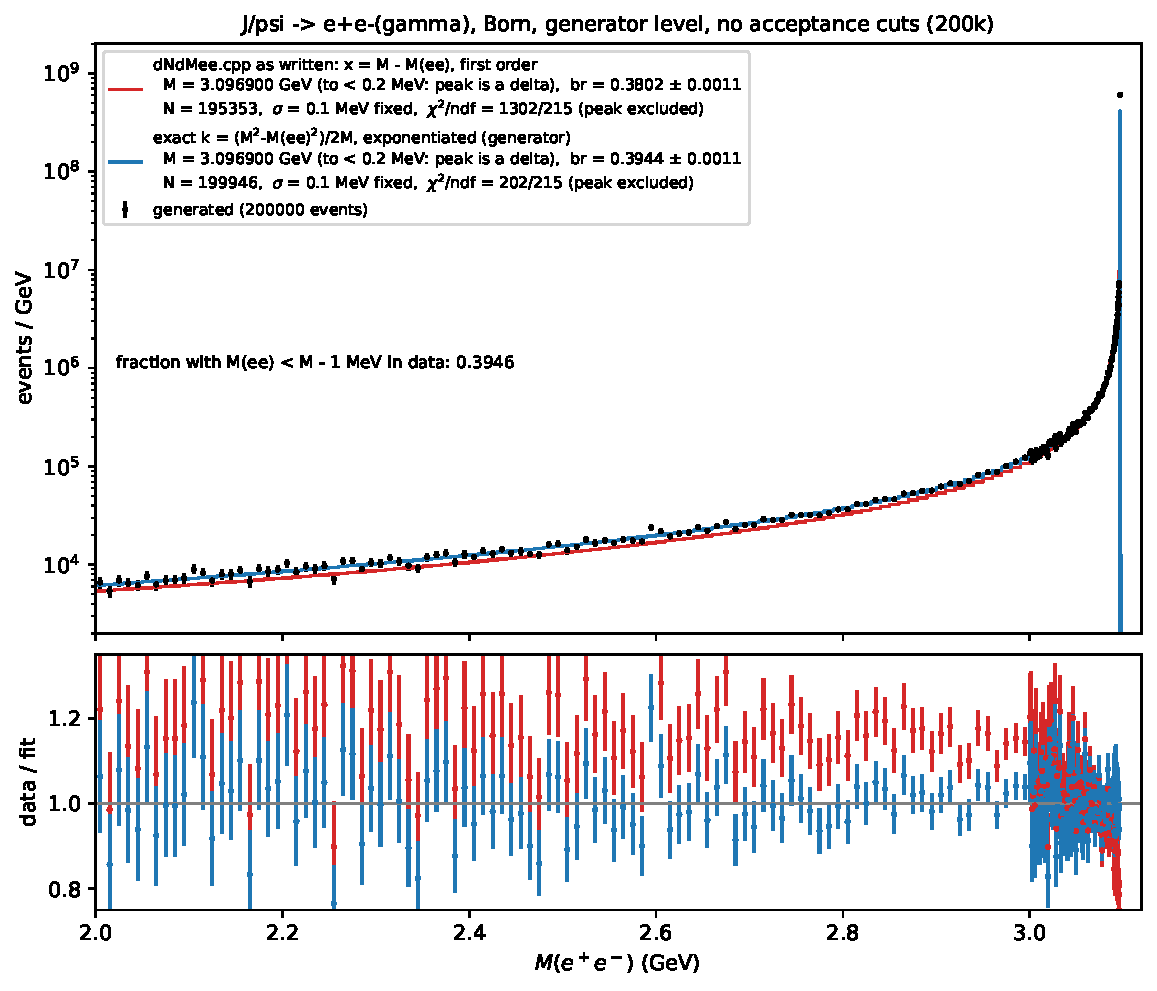
\includegraphics[width=0.72\textwidth]{figures/fig_truth_fit.pdf}
\caption{Generator-level $\Mee$ with the original (red) and the exact (blue) model;
lower panel data/fit.}
\label{fig:truth}
\end{figure}

The same MC truth, without any resolution and with no free parameter in v2
($N$ = number of generated decays, \texttt{br} = QED), is shown in
Fig.~\ref{fig:nores} against $\Delta M=M-\Mee$ in log bins.  The generator's
threshold $\varepsilon=1$~MeV is directly visible: 121\,083 decays (0.6054) sit
exactly at $M$, against $F(1~\text{MeV})=0.6055$ (121\,102 expected); not a
single event lies between $\Delta M=0$ and $\Delta M(k{=}\varepsilon)=1.0002$~MeV;
above it v2 describes the tail over three decades of $\Delta M$ with
$\chi^2$/ndf = 50/61.  The original function, even at its own best fit, is
20\,\% low at $\Delta M=1$--3~MeV and 15\,\% high above 0.3~GeV --- the $1/k$
first-order spectrum with $k$ replaced by $M-\Mee$.

\begin{figure}[p]
\centering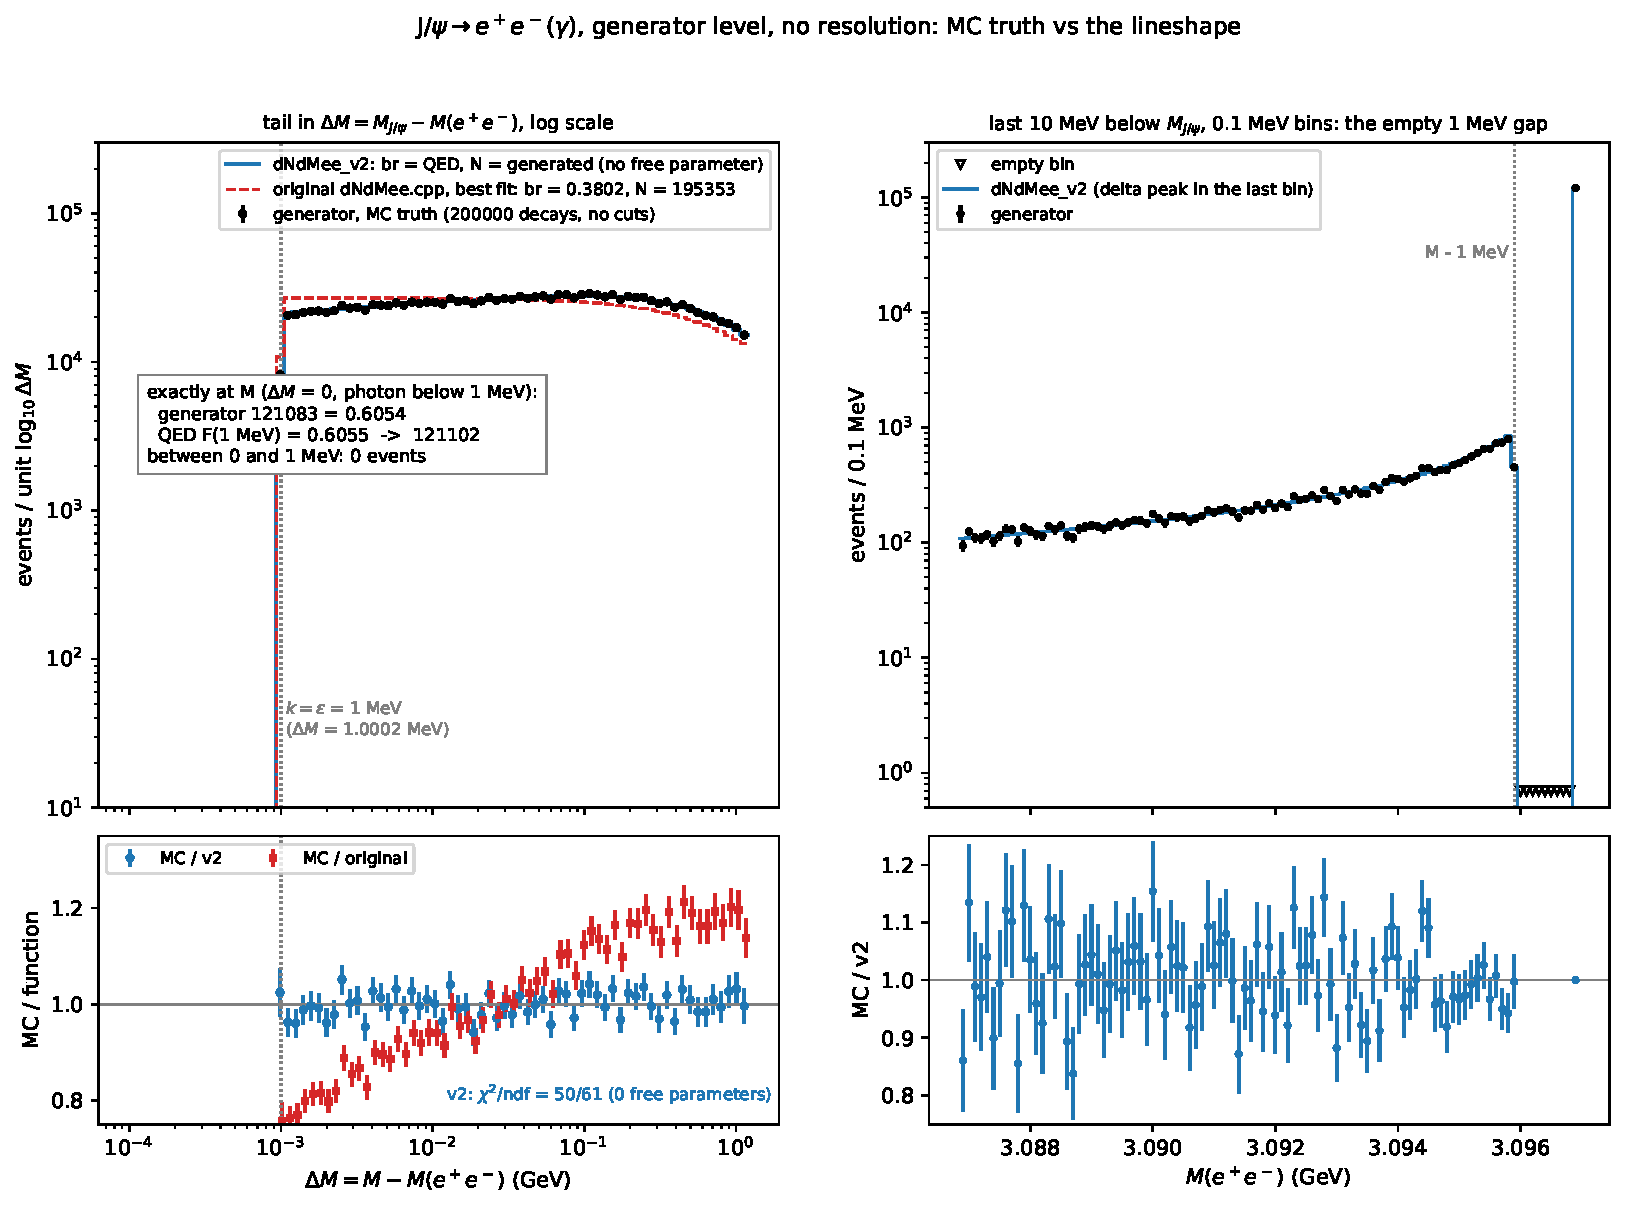
\includegraphics[width=\textwidth]{figures/fig_truth_nores.pdf}
\caption{MC truth without resolution.  Left: tail in $\Delta M=M-\Mee$ (log bins),
v2 with no free parameter and the original function at its best fit.  Right: the
last 10~MeV below $M$ in 0.1~MeV bins: the empty 1~MeV gap and the delta peak.}
\label{fig:nores}
\end{figure}

\subsection{Pseudo-data: MC truth folded with a Gaussian}
\textbf{No GEMC and no data are used in this section.}  The input is the generator's
own $\Mee$ (the 200k events of the previous section); each event is shifted by a
random number drawn from a Gaussian of width $\sigma_{\rm true}=30$ or 50~MeV.  This
is an idealised detector with a known answer: $M=3.0969$~GeV, $\sigma=\sigma_{\rm true}$, $N=200\,000$ (the function is
normalised over all $\Mee$, so $N$ is the total number of decays even though the fit
range is 2.6--3.3~GeV).

\begin{center}
\begin{tabular}{llcccc}\toprule
$\sigma_{\rm true}$ & fit & $M$ (GeV) & $\sigma$ (MeV) & $N$ & \texttt{br} \\\midrule
30 MeV & F1: v2, br = QED   & 3.09685 & $29.92\pm0.07$ & $199\,890\pm460$ & 0.3945 fixed\\
       & F2: v2, br free     & 3.09692 & $29.89\pm0.07$ & $199\,980\pm470$ & $0.398\pm0.003$\\
       & F3: original, br free & \textbf{3.09762} & 29.73 & $\mathbf{195\,035}$ & \textbf{0.438}\\\midrule
50 MeV & F1: v2, br = QED   & 3.09679 & $49.91\pm0.11$ & $199\,940\pm460$ & 0.3945 fixed\\
       & F2: v2, br free     & 3.09700 & $49.83\pm0.12$ & $200\,100\pm470$ & $0.400\pm0.003$\\
       & F3: original, br free & \textbf{3.09790} & 49.64 & $\mathbf{195\,120}$ & \textbf{0.446}\\\bottomrule
\end{tabular}
\end{center}
$\chi^2$/ndf is 125/120 (F1), 123/119 (F2) and 137/118 (F3) at 30~MeV and 125/134,
121/133, 122/132 at 50~MeV: \textbf{the original function fits as well as the correct
one}, while it loses 2.5\,\% of the yield and shifts $M$ by +0.7--1.0~MeV.  The
corrected function returns all three quantities without bias, and a free
\texttt{br} comes out at the QED value.

\begin{figure}[p]
\centering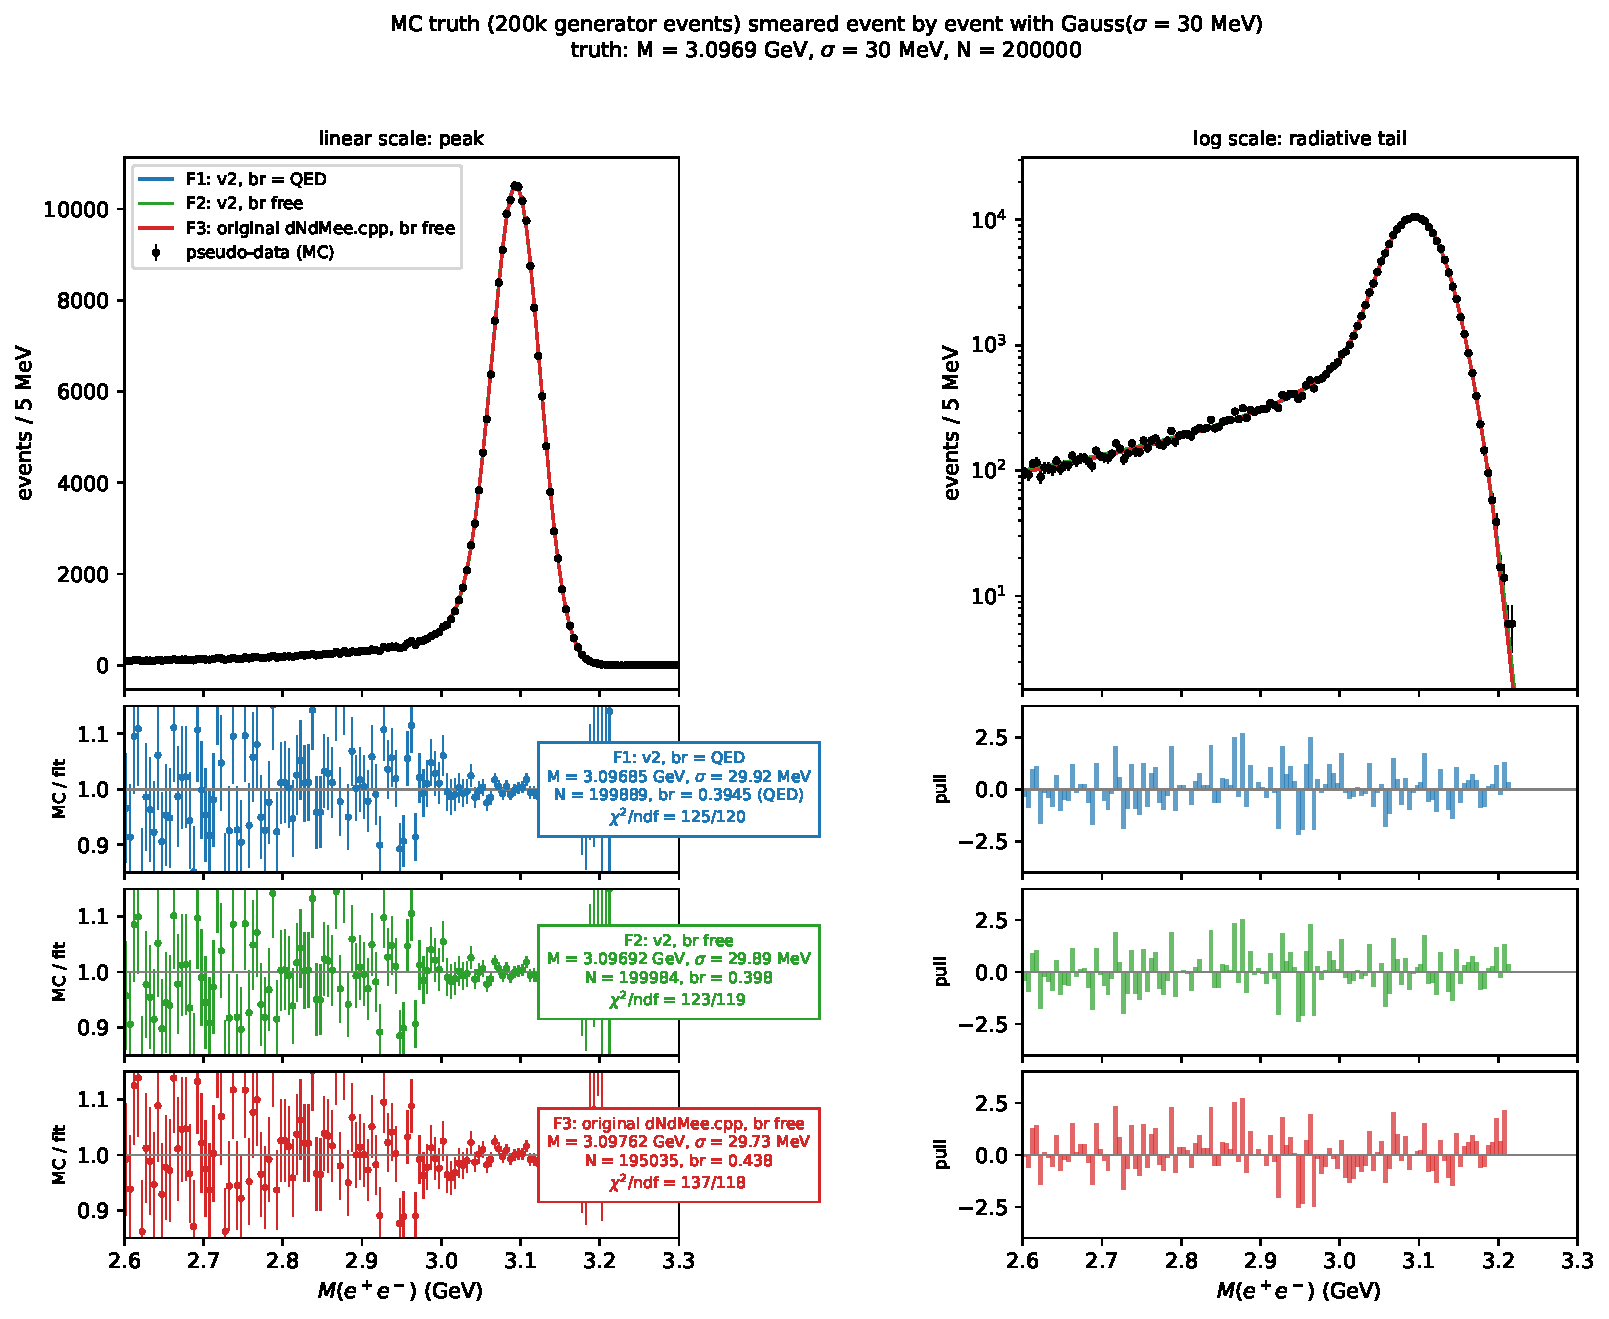
\includegraphics[width=\textwidth]{figures/fig_fit_smeared_30.pdf}
\caption{How the three fits lie on the MC: pseudo-data ($\sigma_{\rm true}=30$~MeV)
in linear and log scale, and for each fit MC/fit and the pull per bin.  All three
describe the MC within statistics; F3 does it with the wrong $M$ and $N$.}
\label{fig:smeared}
\end{figure}

\begin{figure}[p]
\centering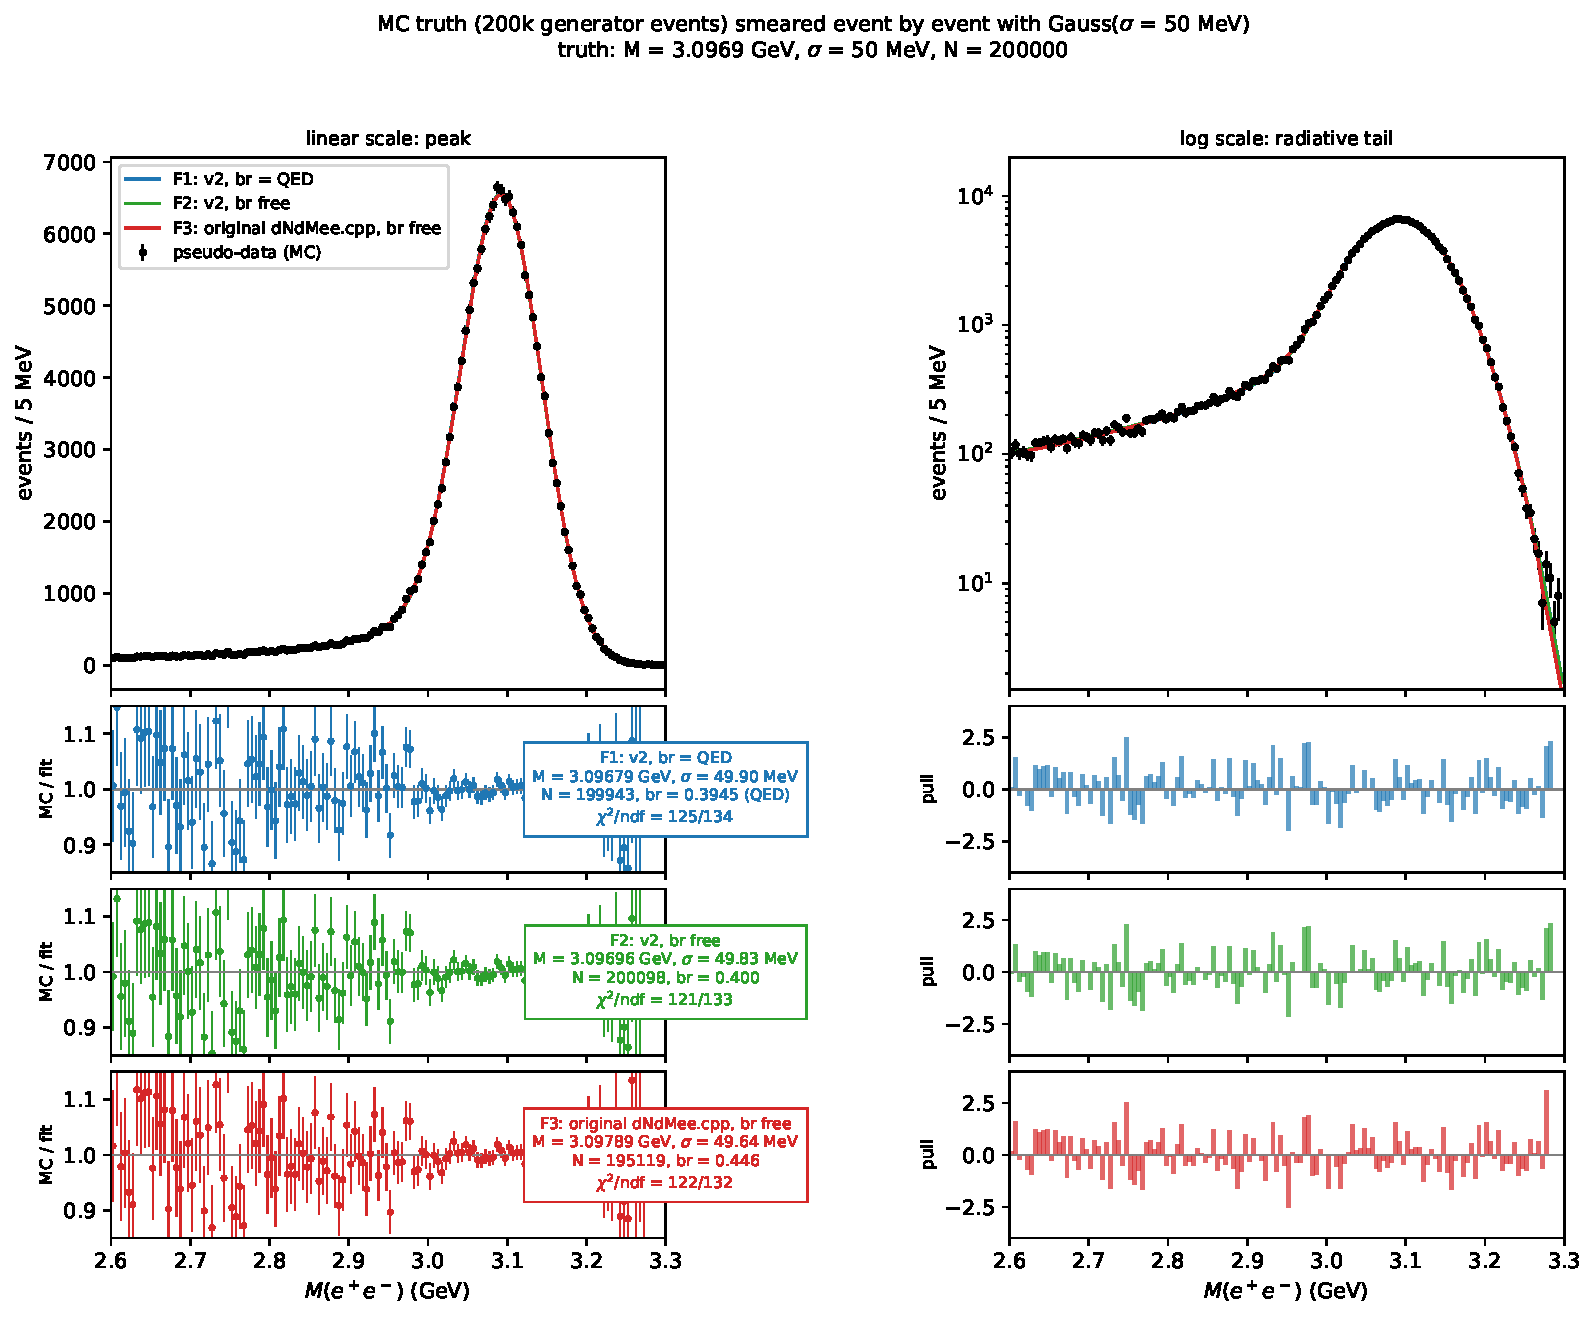
\includegraphics[width=\textwidth]{figures/fig_fit_smeared_50.pdf}
\caption{As Fig.~\ref{fig:smeared}, $\sigma_{\rm true}=50$~MeV.}
\label{fig:smeared50}
\end{figure}

\subsection{Dependence on $\varepsilon$}
With \texttt{br} fixed to $1-F(\varepsilon)$ at every $\varepsilon$
(Fig.~\ref{fig:eps}): $\sigma$ stays at 30.02--30.05~MeV and $\chi^2$ at 116--117/120
for $\varepsilon=0.1\ldots10$~MeV, while \texttt{br} itself moves from 0.49 to 0.28
--- it is a bookkeeping split, not a physics parameter.  $M$ shifts by $-0.25$~MeV
at $\varepsilon=5$~MeV and $-0.55$~MeV at 10~MeV, because decays with a photon below
$\varepsilon$ are put exactly at $M$; it is stable within 0.06~MeV for
$\varepsilon\le1$~MeV.

\begin{figure}[h]
\centering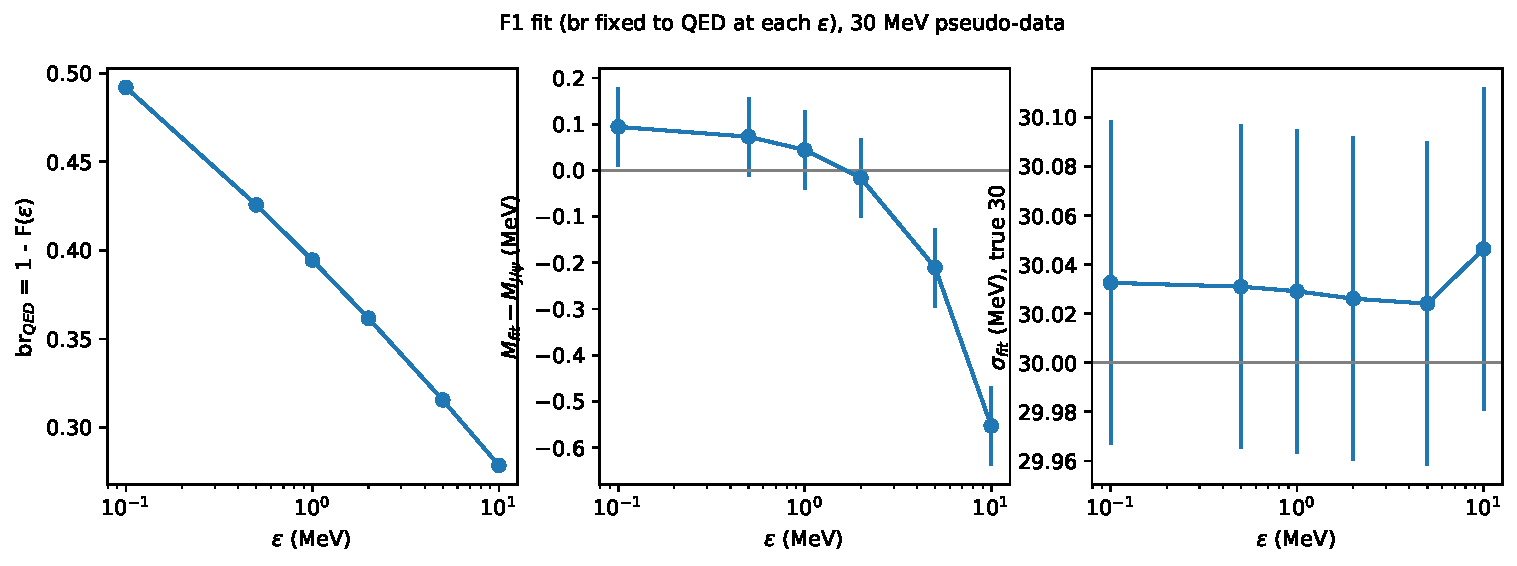
\includegraphics[width=\textwidth]{figures/fig_eps_scan.pdf}
\caption{QED \texttt{br}, fitted $M$ and fitted $\sigma$ against $\varepsilon$.}
\label{fig:eps}
\end{figure}

\subsection{Lepton acceptance}
The 1M Born sample of the f18in production carries the generator's lepton cuts
(\texttt{iacc jpsi}).  Folded with 30~MeV: F1 gives $M=3.09697$~GeV,
$\sigma=29.95\pm0.03$~MeV, $\chi^2$/ndf 117/122; a free \texttt{br} gives
$0.3949\pm0.0011$, the QED value.  The cuts remove radiative decays slightly more
often (13.8\,\% below 3.0~GeV instead of 14.7\,\% in that sample) but do not change
the shape a fit sees (Fig.~\ref{fig:prod}).

\begin{figure}[p]
\centering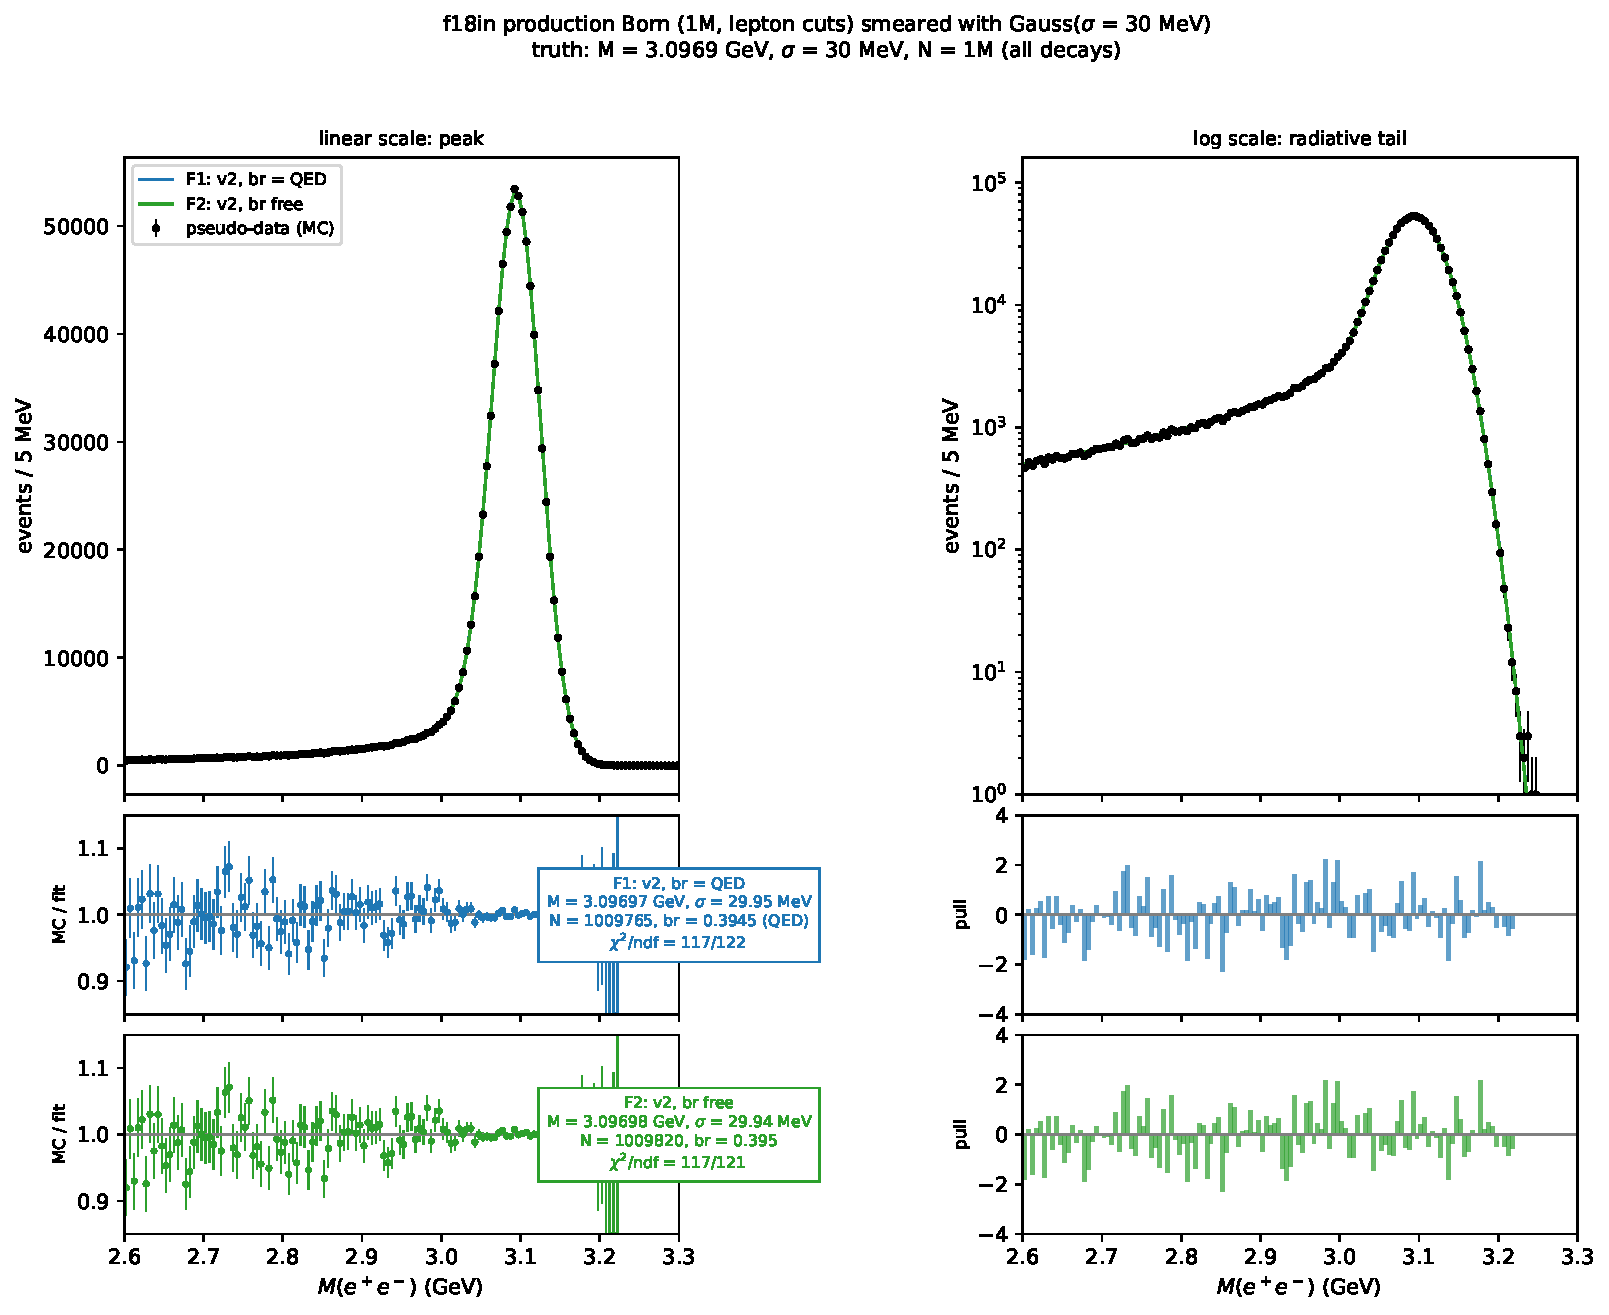
\includegraphics[width=\textwidth]{figures/fig_fit_prod_30.pdf}
\caption{F1 and F2 on the 1M f18in production Born sample (generator lepton cuts),
smeared with 30~MeV.}
\label{fig:prod}
\end{figure}

\section{Recommendation for fitting data}

\begin{enumerate}
\item \textbf{Do not fit the radiative part.}  Use \texttt{dNdMee\_v2} with
  \texttt{br}~$<0$: the fraction and the shape of the radiative tail are QED, fixed
  by $M$ and $m_e$, and validated against the generator to five digits.  Freeing
  \texttt{br} adds nothing (it returns the QED value) except a correlation with the
  resolution.  This is the ``fix the MC parameters, then fit only the resolution''
  idea, with the MC parameters replaced by their exact values.
\item \textbf{Free parameters on data:} the yield $N$, the mass $M$ (in practice the
  momentum scale), the resolution $\sigma$, and the background.
\item \textbf{$\varepsilon$:} keep 1~MeV (or anywhere in 0.1--1~MeV).  Moving it does
  not change the fit as long as $\varepsilon\ll\sigma$ and \texttt{br} follows it,
  which v2 does automatically; above $\sim$5~MeV $M$ starts to be pulled.
\item \textbf{The yield} $N$ is the total number of $\Jpsi\to e^+e^-(\gamma)$ decays
  over all $\Mee$; divide it by the PDG branching ratio with no extra $1+\delta$.
\item \textbf{Do not use the original \texttt{dNdMee.cpp} for yields}: its 2.5\,\% loss
  is invisible in $\chi^2$.
\end{enumerate}

\textbf{What a Gaussian does not cover.}  The real detector adds its own low-mass tail
(bremsstrahlung of the leptons in the target and in the material before the drift
chambers), shifts the momentum scale (the 200-event GEMC test of 8 October showed
lepton momenta 1.4\,\% low), and is not Gaussian in the tails.  Fitting data with a
Gaussian $\sigma$ alone would push that detector tail into $N$ and $M$.  The next
step is therefore GEMC: take the reconstructed-minus-generated $\Mee$ of each event
from the f18in production, parametrise the response (Gaussian core plus a low-side
tail), and fit data with
\[
  \frac{dN}{d\Mee} = N\,\Big[\text{QED (fixed)} \otimes
  \text{detector response (shape from GEMC, scale and width free)}\Big]
  + \text{background}.
\]
For the yield the most robust alternative is a template fit with the GEMC
reconstructed $\Mee$ of the Born and radiative samples directly.

\section*{Files}
Branch \texttt{mee-lineshape} of \texttt{jpsi-rc-2026}, directory \path{mee_lineshape/}:
\begin{itemize}
\item \path{dNdMee_v2.cpp} --- the function;
\item \path{study_lineshape.py} --- all fits, through the compiled library;
\item \path{make_figures_mee.py}, \path{make_truth_nores.py} and this report.
\end{itemize}
Inputs: 200k Born generator events (exclurad\_py, card \path{born_jpsi.txt}, model
\path{jpsi.diffrad_vm_pdet}, \texttt{iacc none}) in
\path{/Volumes/wd_14tb/jpsi_electro_rc/mee200k_0956}, and the 1M Born sample in
\path{/volatile/clas12/vpk/prod_jpsi_f18in_20261009}.

\end{document}
